
\section{Methodology}

\subsection{Overall Architecture}

\begin{figure*}
    \centering
    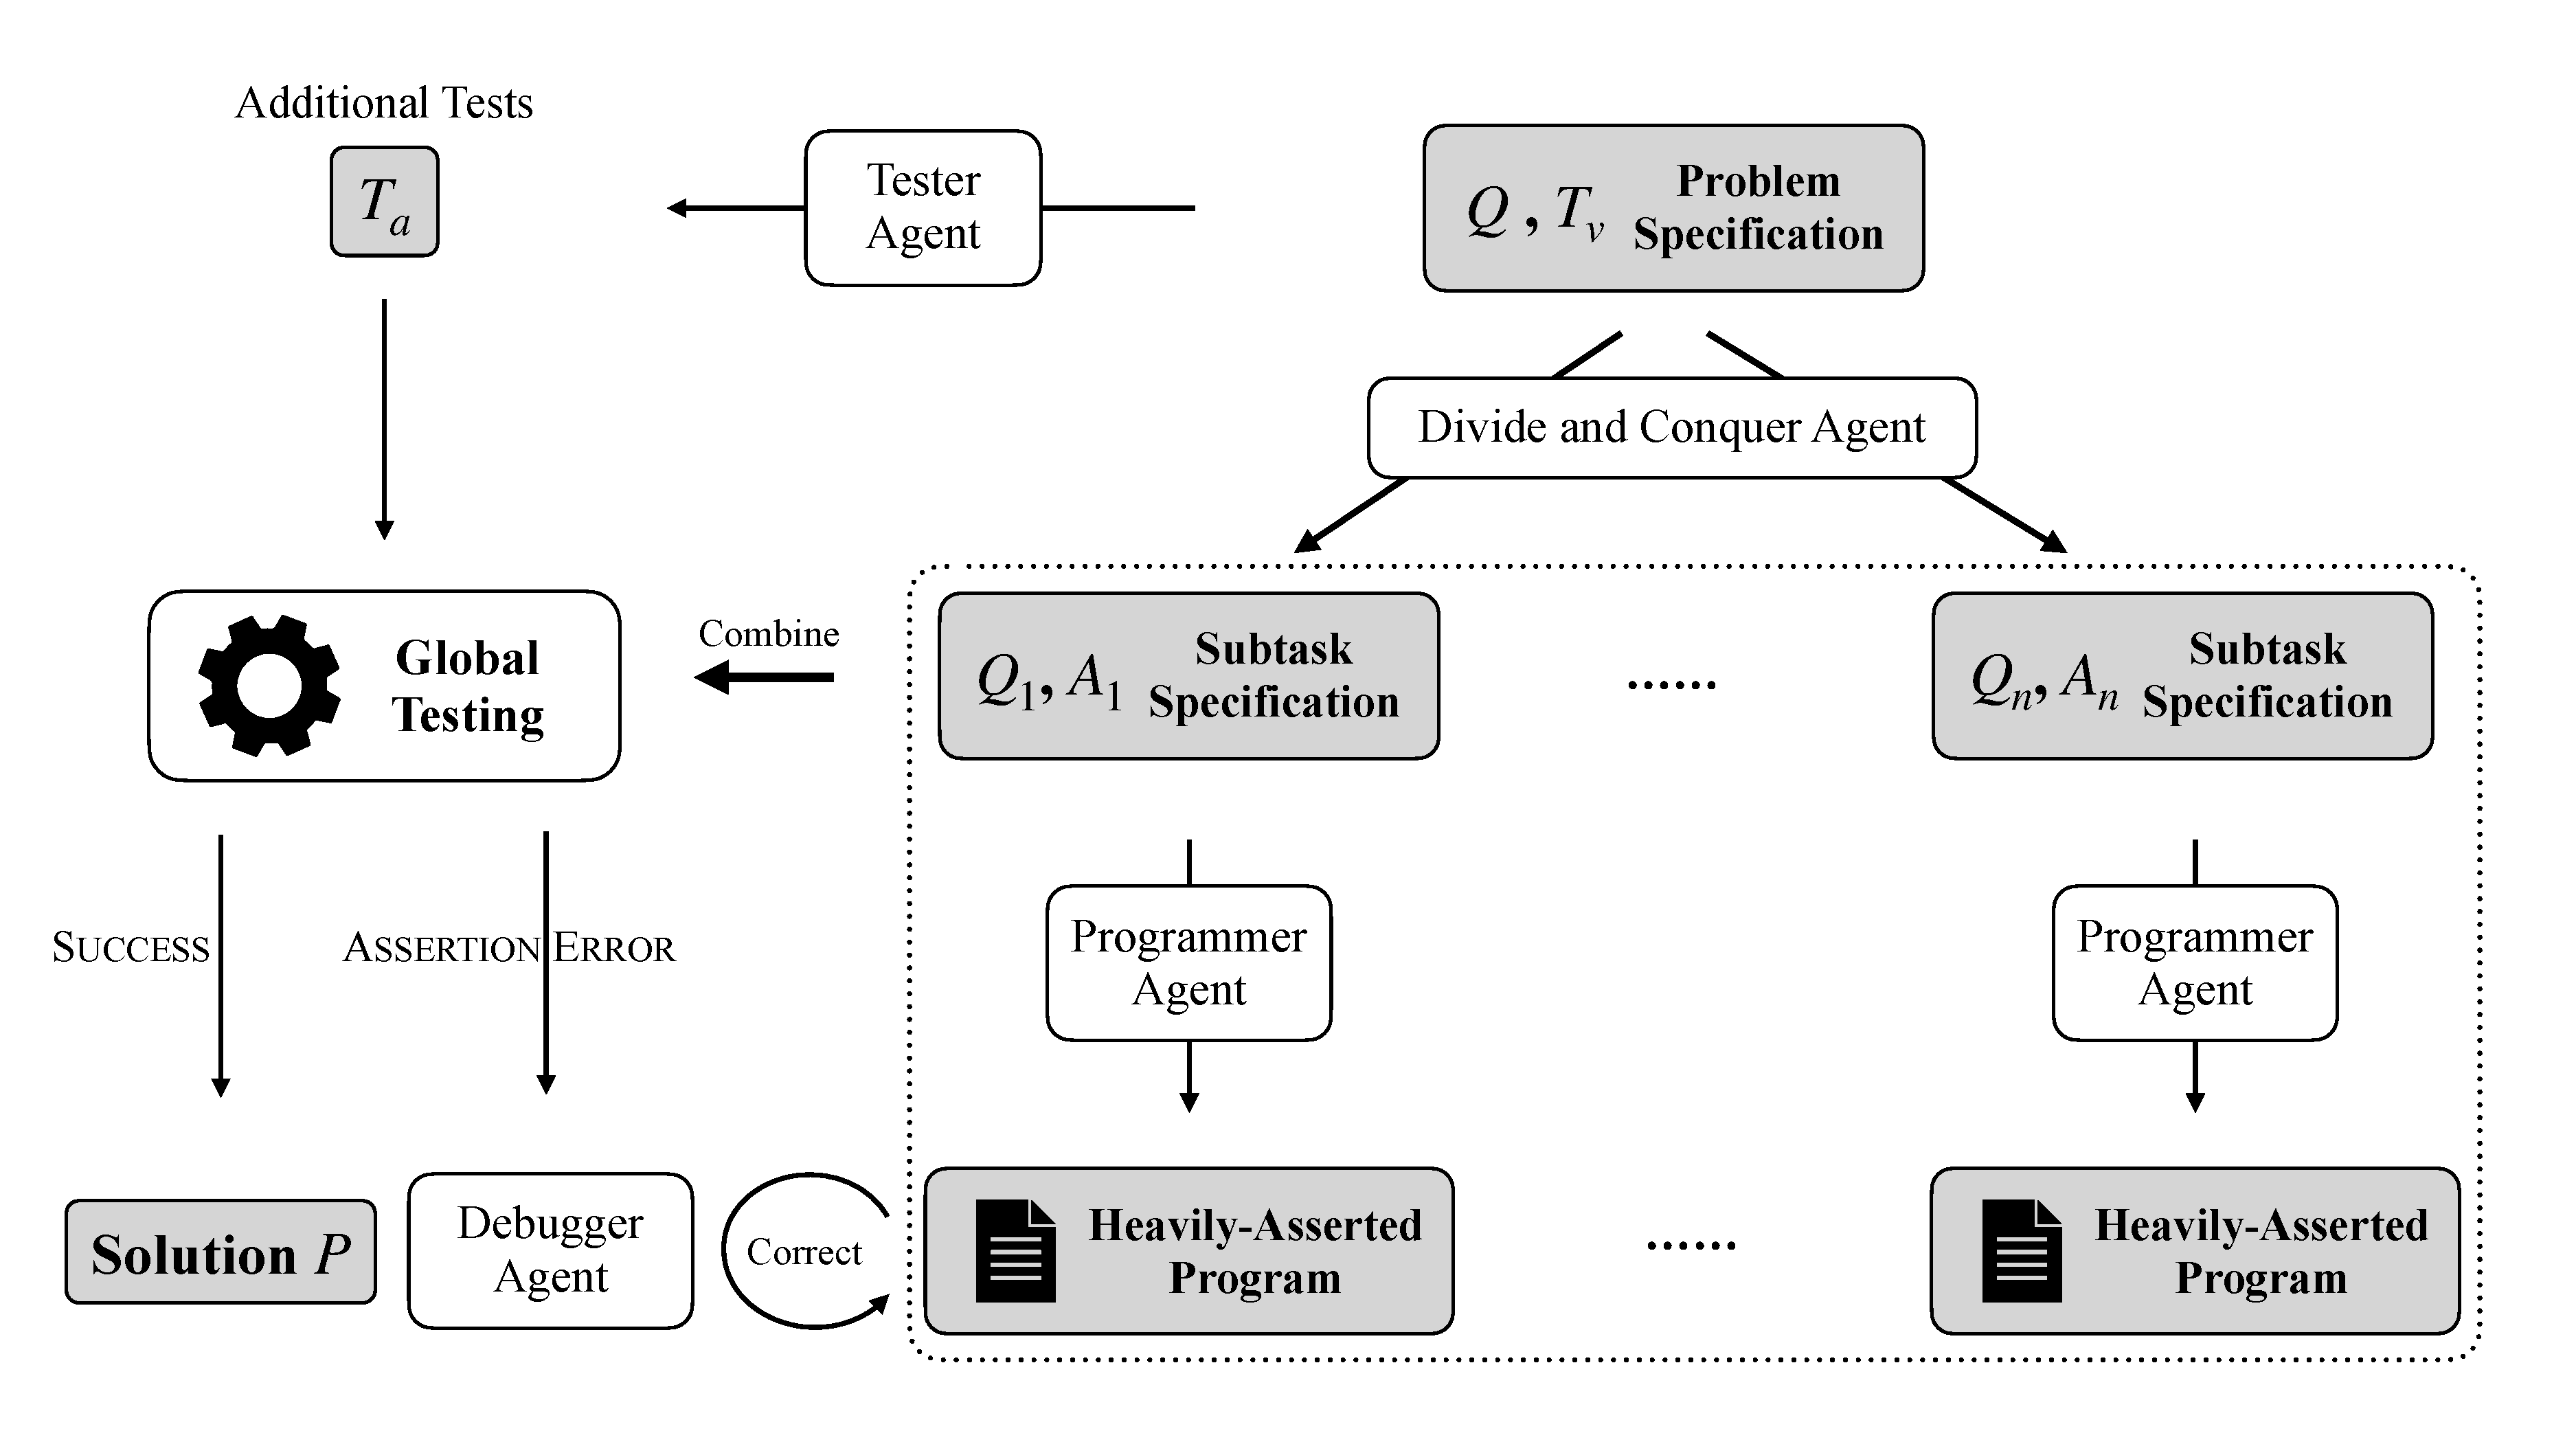
\includegraphics[width=\linewidth]{Architecture.pdf}
    \caption{Overview of the proposed assertion-based debugging framework.}
    \label{fig:overview}
\end{figure*}

Figure~\ref{fig:overview} illustrates an assertion-based debugging framework for large language models (LLMs), which adopts a divide-and-conquer strategy for both problem-solving and debugging. The process begins with a divide-and-conquer agent that decomposes the overall problem specification into a set of smaller subtask specifications. Each subtask is represented as a pair $(Q_i, A_i)$, where $Q_i$ is a natural language description of the subtask, and $A_i$ is a set of assertions that any valid solution must satisfy.

In addition to generating these subtasks, the divide-and-conquer agent also produces the code required to assemble the individual subprograms into a unified solution. Each subtask is then handled by a programmer agent, which implements a corresponding function enriched with detailed runtime assertions. These assertions are designed to catch potential errors and enforce the correctness of the solution.

To verify the correctness of the assembled program, a tester agent generates a single unit test function. This function combines predefined and automatically generated test cases to evaluate the entire solution in a global testing phase. If all tests pass, the solution is accepted. Otherwise, if an assertion fails, a debugger agent is invoked.

The debugger agent is the core of this framework. It analyzes the error message to locate the source of the bug by navigating the codebase. Once sufficient information is gathered, it proposes a fix by replacing one or more faulty functions with corrected versions. The testing and debugging cycle continues iteratively until a correct solution is found. This framework mirrors expert-level debugging practices by embedding assertions, systematically isolating faults, and refining the solution step by step.

In some cases, the debugger agent may be unable to localize the issue based solely on the error message—typically due to a misunderstanding of the original problem specification. When this occurs, the entire process is restarted from scratch to produce a new candidate solution.

% It is worth noting that, the debugger agent, the tester agent and the programmer agents in the framework can work \textit{concurrently} without depending on the completion of each other. This parallel processing capability enhances the efficiency and scalability of the framework, enabling rapid debugging and solution generation for complex programming tasks. The framework's modular design allows for easy integration of additional agents or functionalities, making it adaptable to diverse programming scenarios.

\subsection{Prompt Design}

Since the proposed framework requires a large amount of assertions to generated by the programmer agent, the prompt used to guide the LLMs must be carefully designed to produces desired assertions. We must specify exactly what kind of assertions we want the LLMs to generate, and how to incorporate these assertions into the generated code. The prompt design should also consider the balance between the number of assertions and the complexity of the generated code, as an excessive number of assertions may lead to code bloat and performance degradation.

Here I list the important categories of assertions that I aim to specify in the prompt:

\begin{enumerate}
    \item \textbf{Input Assertions} specify the constraints that the input data must satisfy. These assertions are especially useful for checking the correctness of the combination program generated by the divide-and-conquer agent.
    \item \textbf{Output Assertions} specify the expected output of the program. A lot of engineering efforts need to put into those assertions, as they are the most important part of the program. Thus I force the model to generate such assertions, and recommand the model to create helper functions to check the output match the specialization exactly. For example, in a sorting algorithm, an output assertion may specify that the output list must be sorted in ascending order, which may involves a helper function \texttt{isSorted} to ensure that list is completely sorted.
    \item \textbf{Loop Invariants} can potentially help the model to understand the loop structure and the expected behavior of the loop without using information from long-distance context, and thus generate more accurate assertions. 
\end{enumerate}

Similarly, the prompting strategies used for both the tester agent and the debugger agent play a crucial role in the success of the framework. As illustrate in Figure~\ref{fig:program} one common issue arises when test cases generated by the tester agent are themselves flawed. To mitigate this, I instruct the tester agent to rely primarily on random testing, which helps reduce overfitting to a narrow interpretation of the problem. In this setup, the program specification is effectively written twice: once in the implementation prompt and again in the test generation prompt. This redundancy encourages coverage diversity, but also introduces the potential for misalignment between the two representations of the same task.

Given this setup, the debugger agent must be carefully guided to reason across multiple potential sources of error: the program implementation, the embedded assertions, and the test script itself. It must not only identify the component responsible for the failure but also avoid unnecessarily altering correct parts of the system. To support this, the debugger agent is carefully designed to analyze error messages and assertion failures in a structured manner, navigating the codebase using introspection tools to locate faults. By explicitly including the possibility of errors in any part of the development pipeline—including faulty tests or incorrect assertions - the framework ensures that debugging is not biased toward assuming code is always the source of failure.



